\chapter{Developer Documentation}

In this chapter I will explain what was my plan going into the development of my thesis, how I handled problems during development, and I will finally show the test conducted to compare the libraries.

\section{Development plan}
\label{chap:plan}

For my planing I choose to do my project using the \CC\ programming language. To visualize the data I choose to use \ac{SDL2} with \ac{ImGui} and OpenGL and obviously for \ac{GPGPU} libraries CUDA and OpenCL. The main plan was to implement the two edge detection algorithms. I could have choose to do only the algorithm implementation without a user interface but I decided against it. The reason simply being that goal of the thesis is to show the difference of \ac{GPGPU} libraries speed and be a helpful tool for people to test them out themselves. Thus the plan for the Gui was to have two programs one for synthetic testing environment pure library speed. The result from those test are for pictures that only contain two colors and have simple lines and curves on them. This proves a good way of testing for accuracy and speed but in a real world scenario a real picture could have very different results. Thus the other program's goal is to test real pictures. This program cannot test accuracy and it's main function is to test the speed of the algorithm on a real picture and show the results.


\subsection{Architecture and Classes}
\label{chap:dev}
The plan for the architecture was a simple Model View but its hard to differentiate what's part of a Model and View since there's no library elements or event management system in \CC\ and the aforementioned libraries. The plan was to write an abstraction layer over \ac{SDL2} to use as the base for displaying the \ac{ImGui} and the pictures. Obviously this contains some logic but these logic are mainly related to displaying the images and the Gui.

I will only describe the plans for the picture detector and will only go into the details of the synthetic tester when the plans differed because the basic structure of the two program is the same.

I will only explain the part of the plan for the View which is relevant to the thesis. I use my own \ac{SDL2}-OpenGl pipeline abstraction that is very generalised and could be changed to any library for example Qt to show images and the Gui. I choose to use my own abstraction because I wanted a light weight program and didn't want to depend on a huge library. 

\begin{figure}[H]
\centering
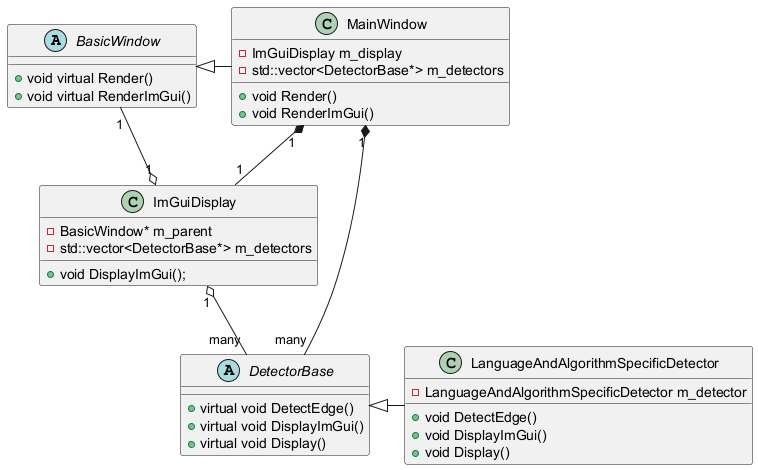
\includegraphics[width=0.8\linewidth]{view}
\caption{Class diagram of view plan}
\label{fig:class_view_plan}
\end{figure}

As I demonstrate in \autoref{fig:class_view_plan} the plan was that I have a basic abstract window class named \textit{BasicWindow} in my own pipeline abstraction and implement a main window from that. Because of the complexity of the ImGui display I choose to use a class to abstract out the common elements. Lastly the detectors themselves are implementing a base class so I can store them in the main window but still have different implementation for all the algorithms in all the languages. This means that I would have six of these classes because of this as I will show later in \autoref{chap:Imp_Arc} this changed while developing and I will explain the reason for it in that subsection. As I have stated above there was no plan for the synthetic tester to have different class structure so the only difference is how the ImGui looks.

As for the models architecturally I use the two libraries that I'm testing to implement the algorithms on the \ac{GPU} and I used no external libraries to implement the algorithm on the \ac{CPU}

\begin{figure}[H]
\centering
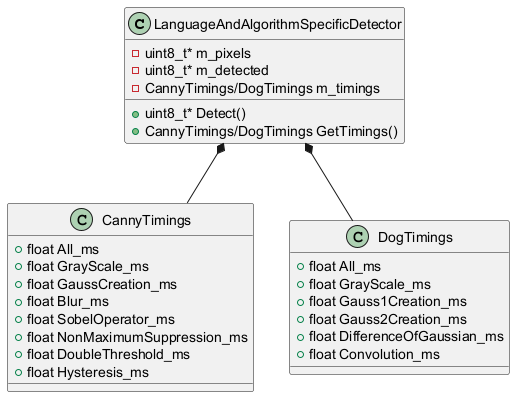
\includegraphics[width=0.8\linewidth]{model}
\caption{Class diagram of model plan}
\label{fig:class_model_plan}
\end{figure}

For the plan of the class structure because on CUDA I need separate functions, and for OpenCl I need separate kernel files, I thought that I cannot abstract out any common element except for the struct for the timings, I choose to just create separate classes for them. As shown on the Class diagram in \autoref{fig:class_model_plan} but as with the View as I started implementing it this planed changed slightly and I will discuss this latter at \autoref{chap:Imp_Arc}.

\subsection{Algorithms}
\label{chap:algo}

So far I only talked about my plans for the view and class structure but by an early stage I know which edge detection algorithms I want to implement and as I have already talked about in \autoref{chap:intro} they are: \ac{Canny} and \ac{DoG}. In this subsection I will demonstrate my plan for the algorithms.

\subsubsection{Canny edge detection}

According to the original article\cite{canny:paper} the \ac{Canny} algorithm has four steps

\begin{enumerate}[nolistsep]
\item Filter out any noise. I choose to use the most popular Gaussian filter for this porous.
\item Find the intensity gradients of the image. For this purpose I use the Sobel filter.
\item Non-maximum suppression. This removes pixels that are not connected to any edge.
\item Hysteresis with double thresh holding. I choose to do this in two steps.
\end{enumerate}

The original article\cite{canny:paper} is very detailed but it's a hard read thus I used other sources\cite{canny:imp}\cite{canny:imp2} to understand the concept better and formulate the algorithms.

Firstly before I can do anything I have to grey scale the image. This is a very simple algorithm as shown in algorithm \ref{alg:grey} I just take the RGB pixel values and multiply them by 0.2999, 0.587, 0.114 accordingly,

\begin{algorithm}[H]
\caption{Grey scaling algorithm}
\label{alg:grey}
\begin{algorithmic}
\State \textbf{Data:} $I$ the RGB pixels of the image
\State \textbf{Result:} $I2$ the grey scaled value of the pixels
\For{$r \; g \; b$ pixel values in $I$ image}
\State $p = 0.299 * r + 0.587 * g + 0.114 * b$
\State where $p$ is the pixel value cores ponding in $I2$
\EndFor
\end{algorithmic}
\end{algorithm}

Now I can focus on the edge detection algorithm properly first is the Gaussian blur. I could use other blurring methods but this is the simplest for our purpose and I can later reuse this in the \ac{DoG} algorithm.

\begin{algorithm}[H]
\caption{Gaussian blur}
\label{alg:gauss}
\begin{algorithmic}
\State \textbf{Data:} $I$ the grey pixels of the image, $G$ the values in the Gaussian kernel in a matrix, $k$ is the size of the kernel
\State \textbf{Result:} $I2$ the output value of the pixels
\For{$c,r$ where $c$ is the index for the column and $r$ is the index for the row of the pixel in $I$ image}
\State $s = 0$
\For{$i=-\frac{k-1}{2},\ldots,\frac{k-1}{2}$}
\For{$j=-\frac{k-1}{2},\ldots,\frac{k-1}{2}$}
\State $s = I[c + i ][r + j] * G[i][j] + s $
\EndFor
\EndFor
\State $I2[c][r] = s$
\EndFor
\end{algorithmic}
\end{algorithm}

In the next step I'm going to calculate the intensity gradient and the edge direction for the image. This step is where I will final get edge lines before this I was only doing preliminary work. The gradient will be our edges and I can calculate the edge directions too which I will use in the next step when I do the Non-maximum suppression to find a single edge line. I use the two directional Sobel filters which are:
\[
\begin{bmatrix}
-1 & 0 & +1 \\
-2 & 0 & +2 \\
-1 & 0 & +1 \\
\end{bmatrix} \qquad
\begin{bmatrix}
+1 & +2 & +1 \\
0 & 0 & 0 \\
-1 & -2 & -1 \\
\end{bmatrix}
\]

\begin{algorithm}[H]
\caption{Intensity gradient}
\label{alg:sobel}
\begin{algorithmic}
\State \textbf{Data:} $I$ the pixels of the image
\State \textbf{Result:} $I2$ the intensity gradient value of the pixels, $I3$ is the edge direction of the pixels
\For{$c,r$ where $c$ is the index for the column and $r$ is the index for the row of the pixel in $I$ image}
\State $SX = \{-1, 0, +1, -2, 0, +2, -1, 0, +1\}$
\State $SY = \{+1, +2, +1, 0, 0, 0, -1, -2, -1\}$
\State $sx = 0$
\State $sy = 0$
\For{$i=-1,\ldots, 1$}
\For{$j=-1,\ldots, 1$}
\State $sx = I[c + i ][r + j] * SX[i][j] + sx $
\State $sy = I[c + i ][r + j] * SY[i][j] + sy $
\EndFor
\EndFor
\State $I2[c][r] = \sqrt{sx^2+sy^2}$
\State $t = \frac{\text{atan2}(sx,sy) * 180}{\pi} $
\If{$t < 180$}
\State $t = t + 180$
\EndIf
\State $I3[c][r] = t$
\EndFor
\end{algorithmic}
\end{algorithm}
\clearpage

Next comes the non maximum suppression in this step I will filter out the gradient so that only continuous edges remain for this purpose I will use the edge direction's I got from the previous step.

\begin{algorithm}[H]
\caption{Non-Maximum suppression}
\label{alg:max}
\begin{algorithmic}
\State \textbf{Data:} $I$ the intensity gradient of the image $I2$ the edge direction of the pixels 
\State \textbf{Result:} $I3$ the pixels of the image that only contain continuous edges
\For{$c,r$ where $c$ is the index for the column and $r$ is the index for the row of the pixel in $I$ image}
\State $q,r = 2000$
\If{$0 \leq I2[c][r] < 22.5$ or $157 \leq I2[c][r] \leq 180$}
\State $q = I[c][r + 1]$
\State $r = I[c][r - 1]$
\ElsIf{$22.5 \leq I2[c][r] < 67.5$}
\State $q = I[c + 1][r - 1]$
\State $r = I[c - 1][r + 1]$
\ElsIf{$67.5 \leq I2[c][r] < 112.5$}
\State $q = I[c + 1][r]$
\State $r = I[c - 1][r]$
\ElsIf{$112.5 \leq I2[c][r] < 157.5$}
\State $q = I[c - 1][r - 1]$
\State $r = I[c + 1][r + 1]$
\EndIf
\If{$I[c][r] \geq q$ and $I[c][r] \geq r$}
\State $I3[c][r] = I[c][r]$
\Else
\State $I3[c][r] = 0$
\EndIf
\EndFor
\end{algorithmic}
\end{algorithm}

The next step I choose to do separately into two separate because of the nature of the  algorithms but in reality they are just one the hysteresis. In the first step the double thresh holding where I categorize the edges into two groups weak edges and strong edges. Based on this then I take all the weak pixels and transform them into strong pixels only in the case when the week pixel have atleast one strong pixel sounding it.

\begin{algorithm}[H]
\caption{Double threshold}
\label{alg:thresh}
\begin{algorithmic}
\State \textbf{Data:} $I$ the pixels of the image, $l$ the low threshold, $h$ the high threshold
\State \textbf{Result:} $I2$ the week and strong pixels of the image
\For{$c,r$ where $c$ is the index for the column and $r$ is the index for the row of the pixel in $I$ image}
\If{$I[c][r] \geq h$}
\State $I2[c][r] = 255$
\ElsIf{$h > I[c][r] \geq l$}
\State $I2[c][r] = 125$
\Else
\State $I2[c][r] = 0$
\EndIf
\EndFor
\end{algorithmic}
\end{algorithm}

\begin{algorithm}[H]
\caption{Hysteresis}
\label{alg:hys}
\begin{algorithmic}
\State \textbf{Data:} $I$ the pixels of the image
\State \textbf{Result:} $I2$ the final image
\For{$c,r$ where $c$ is the index for the column and $r$ is the index for the row of the pixel where $I[c][r] = 125$}
\For{$i=-1,\ldots, 1$}
\For{$j=-1,\ldots, 1$}
\State $s =$ false
\If{$I[c + i][r + j] = 255 $}
\State $s$ = true
\EndIf
\EndFor
\EndFor
\If{$s =$ true}
\State $I[c][r] = 255$
\Else
\State $I[c][r] = 0$
\EndIf
\EndFor
\end{algorithmic}
\end{algorithm}

After I'm done with the Hysteresis I'm done with the algorithm and got my final picture.

\subsubsection{Difference of Gaussians}

This algorithm is much simpler then the previous while the \ac{Canny} have a lot of steps to get a fine tuned image it requires a per image fine tuning to get the best results. In comparison to that the \ac{DoG} algorithm requires much less fine toning but its less accurate too.

I basically already wrote the algorithm previously. First I use algorithm \ref{alg:grey} to gray scale the image. Than I only need algorithm \ref{alg:gauss} to use this. The only difference is that instead of supplying the algorithm a normal Gaussian kernel I first take the difference of two Gaussian kernels and I supply that kernel to the function\cite{dog}. The resulting image will contain the edge lines of our image.

\section{Implementation}

\subsection{Architecture and Classes}
\label{chap:Imp_Arc}
When I started to start programming I started following the plans and realized that I overestimated the amount of classes I needed as seen in \autoref{fig:class_view_real}. Instead of using a separate class for each algorithm and library I can use only two classes for the view. Since the algorithms are the same the visualization for them is the same and I only need to use different detectors for the different libraries.

\begin{figure}[H]
\centering
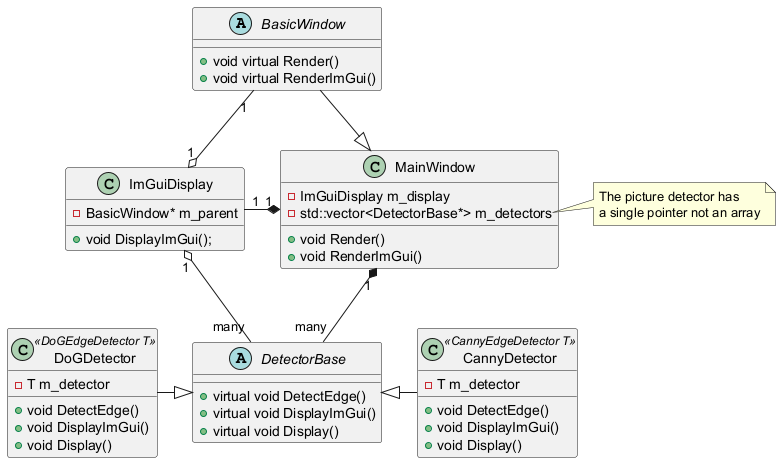
\includegraphics[width=0.8\linewidth]{view_real}
\caption{Class diagram of view implementation}
\label{fig:class_view_real}
\end{figure}

As I show in \autoref{fig:class_view_real} I used \CC\ templates to achieve this. Using this language element I can reuse huge amounts of the code while keeping the View-Model architecture that I defined in \autoref{chap:dev}.

On the other side the model part I needed to make some adjustments as well to accommodate this new design instead of just having all the language and algorithm specific classes there's now a base class. This class abstracts out all the common functionality and defines a virtual function. After this there's two implementation classes of this that further abstracts out things that are common between algorithms. Finally the language specific detectors that only implement the Detect function.

\begin{figure}[H]
\centering
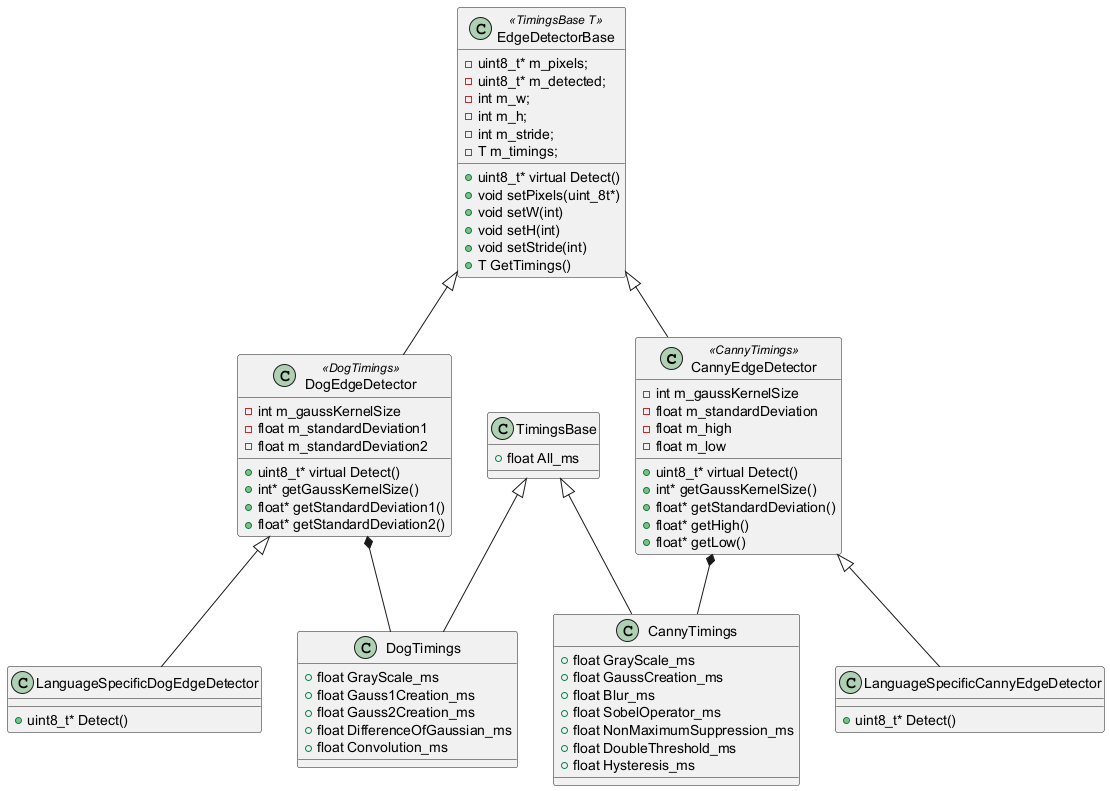
\includegraphics[width=\linewidth]{model_real}
\caption{Class diagram of model implementation}
\label{fig:class_model_real}
\end{figure}

As for the algorithms during implementation there was no need to change anything about them. The only difference between the languages is that on Cuda and OpenCl because they are run on the \ac{GPU} I'm not using double for loops. Instead of for loops in both cases we launch threads grouped into $32 \times 32$ work groups. With this we can maximize the usage of most modern \ac{GPU} which have typically $1024$ threads available. We can use language specific functions to query what number of thread we on whit this we can go over all the pixels in an image much faster then if we used the \ac{CPU}. 


\section{Testing}
\label{chap:dev_testing}

My plans for the testing is simple. Since both programs is designed in a way to compare the algorithms and libraries I will just use them to test the code. Since the visualization is very rudimentary and the code for it is is even simpler there's no need for it to be tested. There's only one vector of failure is that if someone deletes one of the pre defined pictures, OpenCl kernels or OpenGl shaders. These are assumed to exists at all time since the programs cannot function without it.

Some of these tests will be concluded on two machines to compare how hardware effects performance I will not these when it comes up the specifications of the two machines used can be seen in \autoref{tab:machine}. If a test does not state which machine its concluded than it was done on Machine1.

I expect the Cuda version to be the fastest because Cuda has the advantage of only having to build to Nvidia \ac{GPU}. OpenCl will be the second fastest if not in some cases faster since it too runs on the \ac{GPU}. Lastly the \ac{CPU} version while on smaller pictures be fast on larger pictures will fall of rapidly.

\begin{table}[H]
\centering
\resizebox{\textwidth}{!}{\begin{tabular}{| c | c | c | c | c | c | c |}
\hline
Name & Cpu & Gpu & VRam & Ram\\
\hline\hline
Machine1 & AMD Ryzen 9 3900x & Nvidia GeForce RTX 3070 & 8Gb & 32Gb \\
\hline 
Machine2 & AMD Ryzen 5 7535HS & Nvidia GeForce RTX 4050 Laptop & 6Gb & 16Gb\\
\hline
\end{tabular}}
\caption{Specifications of the machines used in testing}
\label{tab:machine}
\end{table}

\subsection{Real picture tester}
\label{chap:reason}

First I will show results about the real picture tester since it is more focused on the visual aspects and not hard data like the synthetic tester. My plans for testing this is to compare bot \ac{DoG} and \ac{Canny} algorithms in all three implementations based on how they look and what we can see as differences and how much time it takes them. As I have mentioned in \autoref{chap:real_pic_tester} I only used pre defined pictures the sizes and names of the pictures are shown below in \autoref{tab:pictures}. I will only show timings if they are relevant but how picture and settings size effect timing will be discussed in \autoref{chap:test_synt_test}.

\begin{table}[H]
\centering
\begin{tabular}{| c | c | c |}
\hline
Name & Width & Height \\
\hline \hline	
gem & 2560 & 1440 \\
\hline
house & 1600 & 1200 \\
\hline
monkey & 7680 & 4320 \\
\hline
lines & 100 & 100 \\
\hline
\end{tabular}
\caption{Pictures used and their sizes}
\label{tab:pictures}
\end{table}

\begin{figure}[H]
\centering
\begin{minipage}[t]{.49\textwidth}
\centering
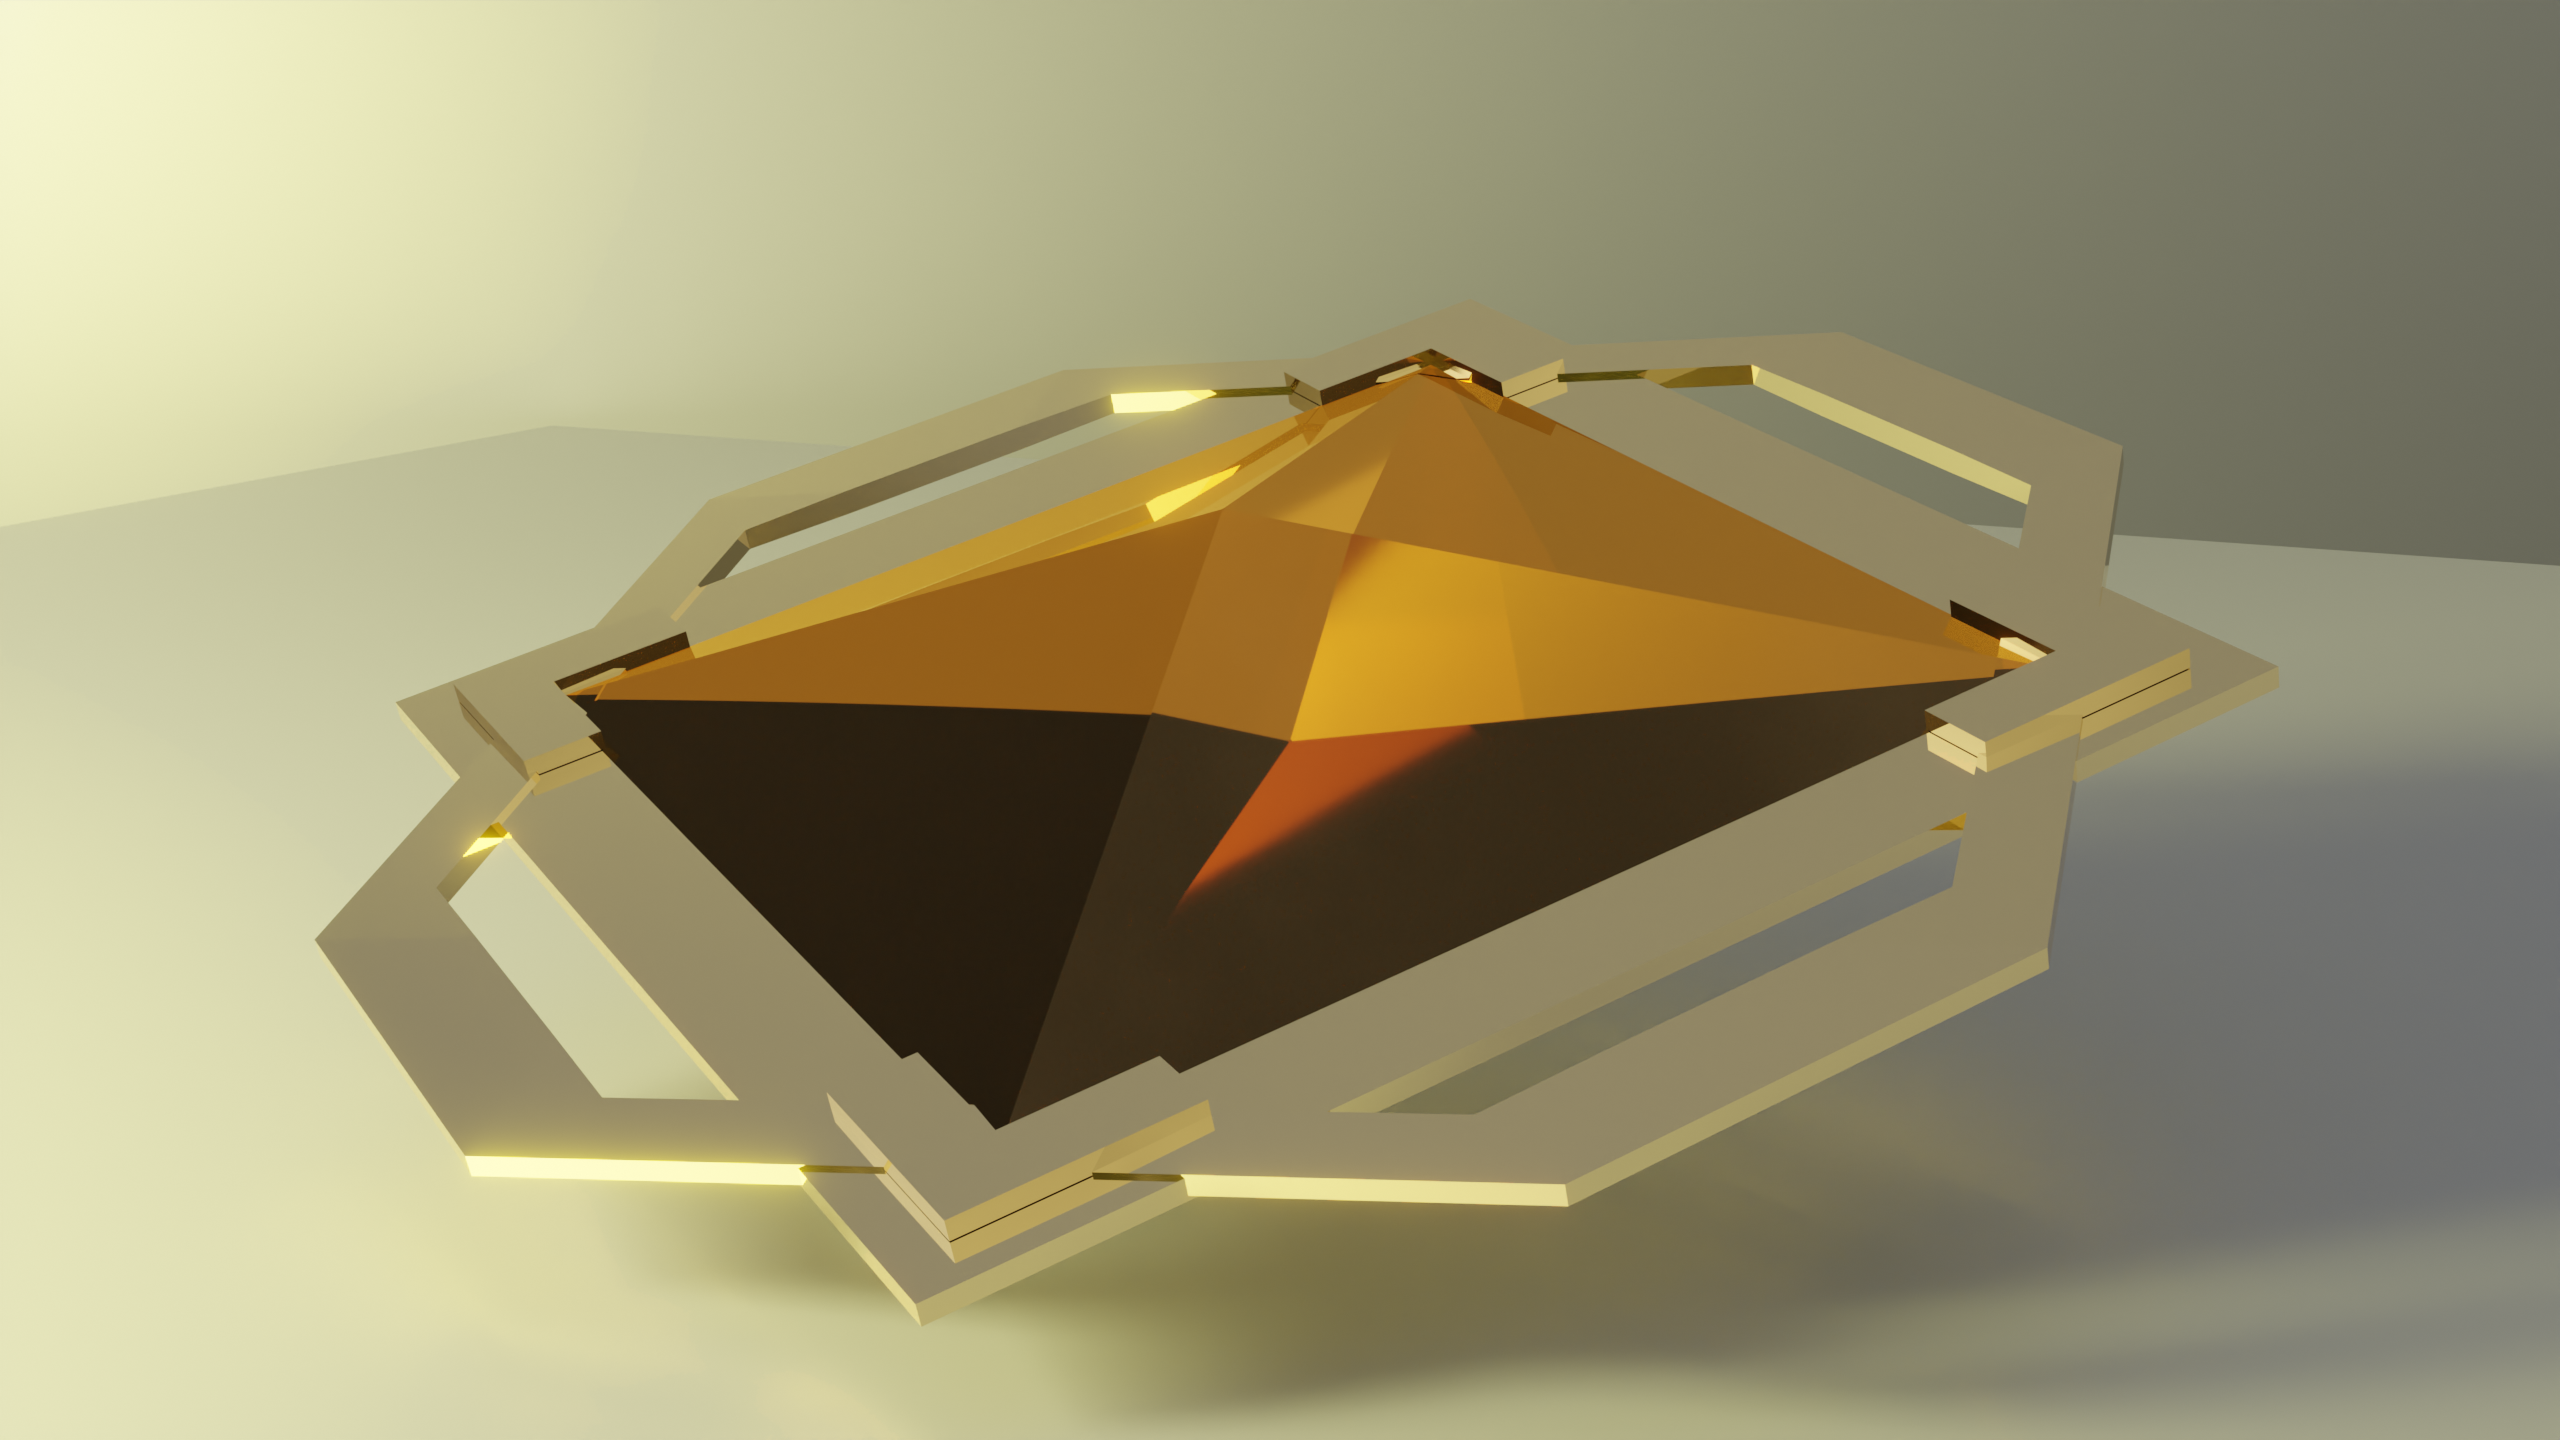
\includegraphics[width=\linewidth]{gem}
\addtocounter{figure}{-1}
\captionsetup{labelformat=empty}
\caption[]{gem}
\end{minipage}
\begin{minipage}[t]{.49\textwidth}
\centering
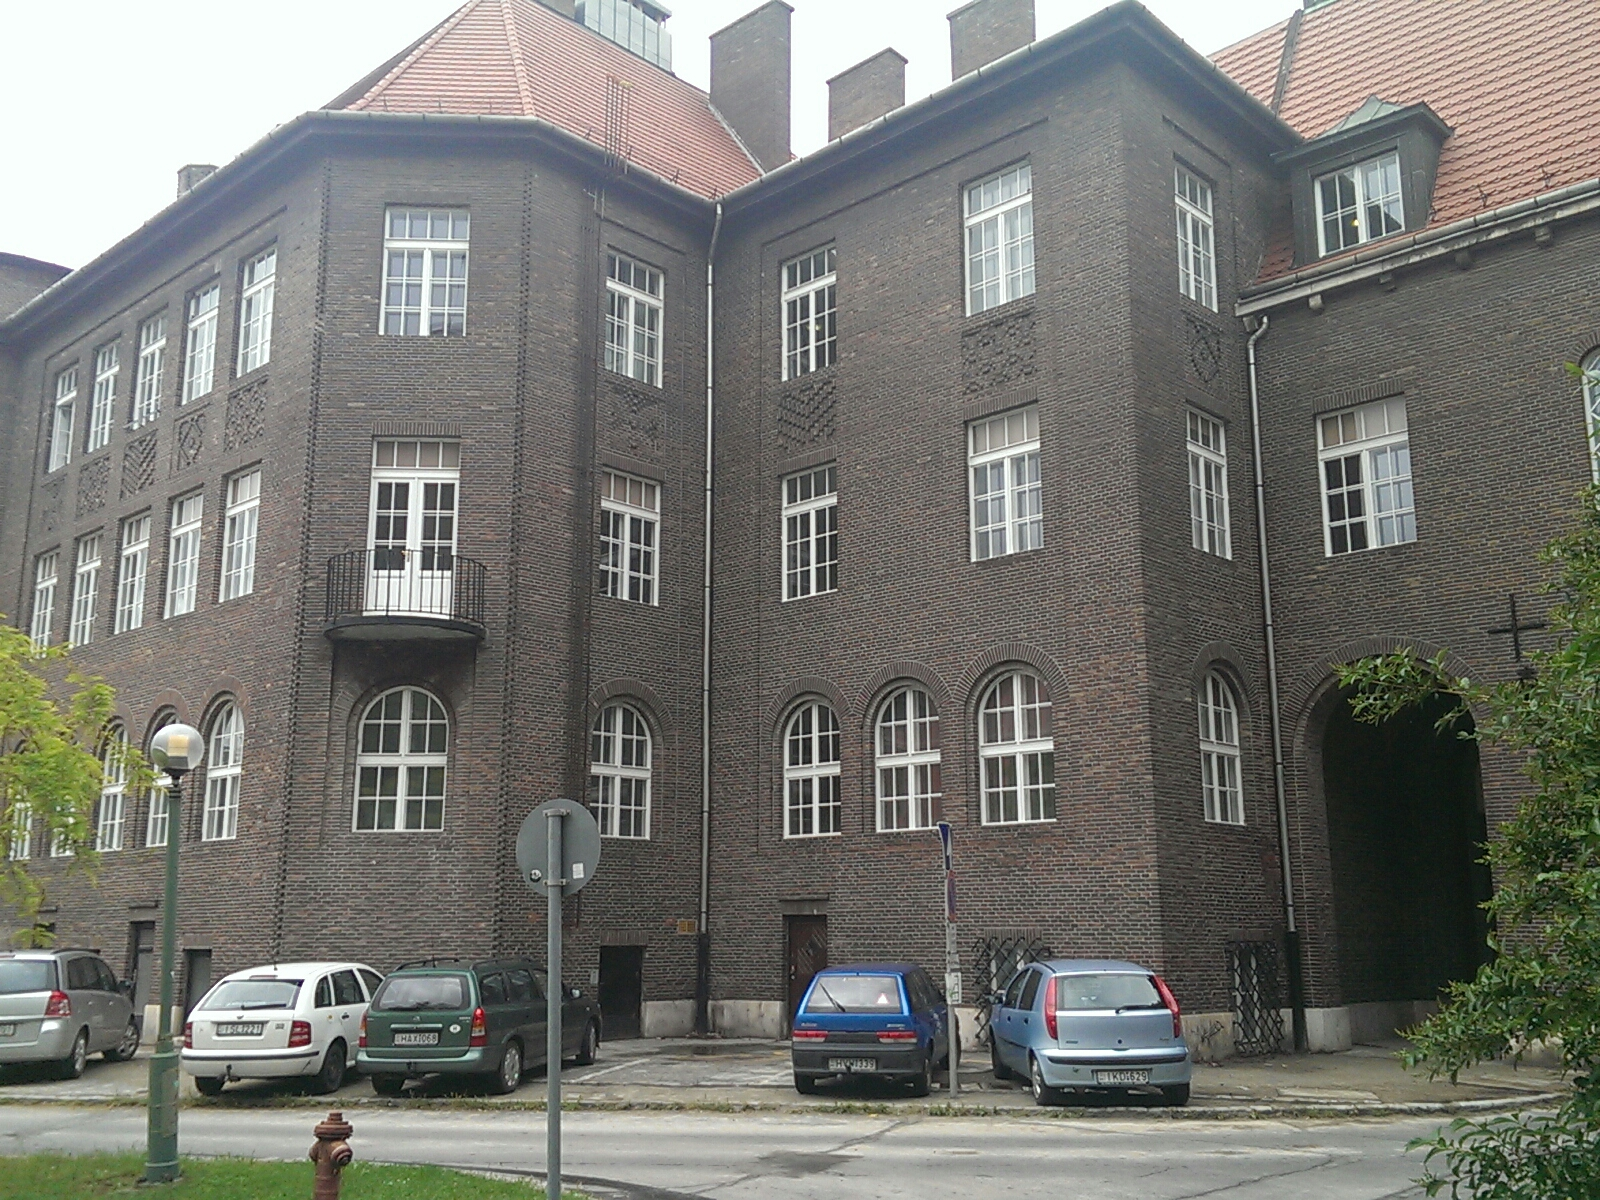
\includegraphics[width=\linewidth]{house}
\addtocounter{figure}{-1}
\captionsetup{labelformat=empty}
\caption[]{house}
\end{minipage}
\begin{minipage}[t]{.49\textwidth}
\centering
\includegraphics[width=\linewidth]{monkey}
\addtocounter{figure}{-1}
\captionsetup{labelformat=empty}
\caption[]{monkey}
\end{minipage}
\begin{minipage}[t]{.49\textwidth}
\centering
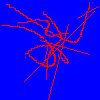
\includegraphics[width=\linewidth, height=.85\linewidth]{lines}
\addtocounter{figure}{-1}
\captionsetup{labelformat=empty}
\caption[]{lines}
\end{minipage}
\caption{The pictures base}
\label{fig:pictures}
\end{figure}

 For this reason I have done quiet a numerous test show in \autoref{tab:real_pic_canny} and \autoref{tab:real_pic_dog}. In the tables I show which picture I used and what settings I set for all three implementations.

\begin{table}[H]
\centering
\resizebox{\textwidth}{!}{\begin{tabular}{| c | c | c | c | c | c |}
\hline
&Name & Gauss kernel size & Standard deviation & High Threshold & Low Threshold\\
\hline\hline
1 & lines & $3$ & $1.0$ & $20.0$ & $10.0$ \\ 
\hline
2 & monkey & $21$ & $1.0$ & $150.0$ & $100.0$ \\ 
\hline
3 & house & $3$ & $1.0$ & $150.0$ & $100.0$ \\
\hline
4 & house & $3$ & $20.0$ & $150.0$ & $100.0$ \\
\hline
5 & house & $11$ & $1.0$ & $150.0$ & $100.0$ \\
\hline
\end{tabular}}
\caption{Test plans for the Real picture tester for \ac{Canny} algorithm}
\label{tab:real_pic_canny}
\end{table}

\begin{table}[H]
\centering
\resizebox{\textwidth}{!}{\begin{tabular}{| c | c | c | c | c |}
\hline
& Name & Gauss kernel size & First standard deviation & Second standard deviation two \\
\hline \hline
1 & lines & $7$ & $0.1$ & $10.0$ \\
\hline
2 & monkey &  $21$ & $0.1$ & $10.0$ \\ 
\hline
3 & lines & $7$ & $0.1$ & $10.0$ \\
\hline
4 & lines & $15$ & $0.1$ & $20.0$ \\
\hline
\end{tabular}}
\caption{Test plans for the Real picture tester for \ac{DoG} algorithm}
\label{tab:real_pic_dog}
\end{table}

The tests in both algorithms case serve to show the same difference so I will explain both of them tougher. The first test is to show what the algorithm looks like exactly this is show in \autoref{fig:test1c}. The slight color difference we can detect in the \ac{DoG} algorithm is because of floating point precisions.


\begin{figure}[H]
\centering
\begin{minipage}[t]{.325\textwidth}
\centering
\includegraphics[width=\linewidth]{test1/canny_cpu}
\addtocounter{figure}{-1}
\captionsetup{labelformat=empty}
\caption[]{Canny Cpu}
\end{minipage}
\begin{minipage}[t]{.325\textwidth}
\centering
\includegraphics[width=\linewidth]{test1/canny_cuda}
\addtocounter{figure}{-1}
\captionsetup{labelformat=empty}
\caption[]{Canny Cuda}
\end{minipage}
\begin{minipage}[t]{.325\textwidth}
\centering
\includegraphics[width=\linewidth]{test1/canny_open_cl}
\addtocounter{figure}{-1}
\captionsetup{labelformat=empty}
\caption[]{Canny OpenCl}
\end{minipage}
\begin{minipage}[t]{.325\textwidth}
\centering
\includegraphics[width=\linewidth]{test1/dog_cpu}
\addtocounter{figure}{-1}
\captionsetup{labelformat=empty}
\caption[]{DoG Cpu}
\end{minipage}
\begin{minipage}[t]{.325\textwidth}
\centering
\includegraphics[width=\linewidth]{test1/dog_cuda}
\addtocounter{figure}{-1}
\captionsetup{labelformat=empty}
\caption[]{DoG Cuda}
\end{minipage}
\begin{minipage}[t]{.325\textwidth}
\centering
\includegraphics[width=\linewidth]{test1/dog_open_cl}
\addtocounter{figure}{-1}
\captionsetup{labelformat=empty}
\caption[]{DoG OpenCl}
\end{minipage}
\caption{Pictures of the first test for real pictures}
\label{fig:test1c}
\end{figure}


\begin{table}[H]
\centering
\resizebox{\textwidth}{!}{\begin{tabular}{| c | c | c | c | c | c | c | c | c |}
\hline
Name & Whole & Grey & Gauss & Blur & Sobel & Non Max & Threshold & Hysteresis \\
\hline \hline
 Canny Cpu& $3.517$ & $0.0525$ & $0.0065$ & $1.1203$ & $1.9339$ & $0.1452$ & $0.0548$ & $0.038$ \\
\hline
 Canny Cuda& $1.10387$ & $0.095232$ & $0.042784$ & $0.047104$ & $0.410624$ & $0.04288$ & $0.0408$ & $0.053248$ \\
\hline
 Canny OpenCl& $9.7643$ & $0.00816$ & $0.006144$ & $0.005184$ & $0.006144$ & $0.006144$ & $0.006144$ & $0.00416$\\
\hline
\end{tabular}}
\resizebox{\textwidth}{!}{\begin{tabular}{| c | c | c | c | c | c | c |}
\hline
Name & Whole & Grey & First Gauss creation & Second Gauss creation & DoG & Convolution \\
\hline \hline
 DoG Cpu& $6.3464$ & $0.0478$ & $0.0056$ & $0.001$ & $0.0003$ & $6.0298$  
 \\
\hline
 DoG Cuda& $0.83456$ & $0.16384$ & $0.044032$ & $0.014336$ & $0.25904$ & $0.062464$  
 \\
\hline
 DoG OpenCl&$4.4794$ & $4.155$ & $0.0661$ & $0.0414$ & $0.0577$ & $0.0599$ 
\\
\hline
\end{tabular}}
\caption{Timings of the first test for real pictures}
\label{tab:test1c}
\end{table}


The first thing to note is that the OpenCl timings will look strange. That's because I used the platform specific timing functions in every case and while Cuda offers a timing method with events. OpenCl on the other hand only offers method to time the execution time of a kernel. This results in the unfortunate fact that the timing whole execution is impossible with platform specific method. For this reason I choose to time it with the chorons built in \CC\ library but this includes the time it took for the kernel to start and other synchronization and function call timing.


\begin{figure}[H]
\centering

\begin{minipage}[t]{.49\textwidth}
\centering
\includegraphics[width=\linewidth]{test2/canny_cuda}
\addtocounter{figure}{-1}
\captionsetup{labelformat=empty}
\caption[]{Canny Cuda}
\end{minipage}
\begin{minipage}[t]{.49\textwidth}
\centering
\includegraphics[width=\linewidth]{test2/dog_cuda}
\addtocounter{figure}{-1}
\captionsetup{labelformat=empty}
\caption[]{DoG Cuda}
\end{minipage}
\caption{Cuda pictures of the second test for real pictures}
\label{fig:test2c}
\end{figure}


\begin{table}[H]
\centering
\resizebox{\textwidth}{!}{\begin{tabular}{| c | c | c | c | c | c | c | c | c |}
\hline
Name & Whole & Grey & Gauss & Blur & Sobel & Non Max & Threshold & Hysteresis \\
\hline \hline
 Canny Cpu& $102957$ & $356.18$ & $0.0046$ & $91340.7$ & $8827.39$ & $866.149$ & $337.775$ & $348.165$\\
\hline
 Canny Cuda&$176.116$ & $8.24525$ & $0.099328$ & $123.817$ & $12.8072$ & $10.753$ & $7.64006$ & $7.6329$ \\
\hline
 Canny OpenCl& $188.599$ & $1.97203$ & $0.017408$ & $28.5286$ & $1.10899$ & $1.01171$ & $0.746592$ & $0.7424$\\
\hline
\end{tabular}}
\resizebox{\textwidth}{!}{\begin{tabular}{| c | c | c | c | c | c | c |}
\hline
Name & Whole & Grey & First Gauss creation & Second Gauss creation & DoG & Convolution \\
\hline \hline
 DoG Cpu& $92683.5$ & $356.98$ & $0.0344$ & $0.0033$ & $0.0032$ & $91244.7$\\
\hline
 DoG Cuda& $118.493$ & $8.02509$ & $0.052224$ & $0.053248$ & $0.420864$ & $108.655$\\
\hline
 DoG OpenCl&$111.162$ & $35.8827$ & $0.1015$ & $0.0544$ & $0.0623$ & $43.9247$ \\
\hline
\end{tabular}}
\caption{Timings of the second test for real pictures}
\label{tab:test2c}
\end{table}

The second tests is the last that we can directly compare the \ac{Canny} and \ac{DoG} implementations. It's main reason is to show the difference between the time it takes for the \ac{CPU} implementations compared to the \ac{GPU} implementations. Due to the size of the original picture the details of the detectors I only show the Cuda versions of the \ac{Canny} and \ac{DoG} pictures. From the third tests forward there will be no timings since I will analyse what impacts timings in details in \autoref{chap:test_synt_test}. Moreover I will use the house picture from going forward since that has the most edge lines from all the pictures. This allowed me to show the differences between the settings and what their impact.

\begin{figure}[H]
\centering
\begin{minipage}[t]{.325\textwidth}
\centering
\includegraphics[width=\linewidth]{test3/canny_cpu}
\addtocounter{figure}{-1}
\captionsetup{labelformat=empty}
\caption[]{Canny Cpu}
\end{minipage}
\begin{minipage}[t]{.325\textwidth}
\centering
\includegraphics[width=\linewidth]{test3/canny_cuda}
\addtocounter{figure}{-1}
\captionsetup{labelformat=empty}
\caption[]{Canny Cuda}
\end{minipage}
\begin{minipage}[t]{.325\textwidth}
\centering
\includegraphics[width=\linewidth]{test3/canny_open_cl}
\addtocounter{figure}{-1}
\captionsetup{labelformat=empty}
\caption[]{Canny OpenCl}
\end{minipage}
\caption{Pictures of the third test in \ac{Canny} for real pictures}
\label{fig:test3c}
\end{figure}

Notice that on the pictures in \autoref{fig:test3c} that the images are very noisy especially the \ac{CPU} picture the differences as I have mentioned before are because of floating point calculation differences between Cuda/OpenCl and normal \CC\ . I will now show two ways as to how to reduce the noise.

\begin{figure}[H]
\centering
\begin{minipage}[t]{.325\textwidth}
\centering
\includegraphics[width=\linewidth]{test4/canny_cpu}
\addtocounter{figure}{-1}
\captionsetup{labelformat=empty}
\caption[]{Canny Cpu}
\end{minipage}
\begin{minipage}[t]{.325\textwidth}
\centering
\includegraphics[width=\linewidth]{test4/canny_cuda}
\addtocounter{figure}{-1}
\captionsetup{labelformat=empty}
\caption[]{Canny Cuda}
\end{minipage}
\begin{minipage}[t]{.325\textwidth}
\centering
\includegraphics[width=\linewidth]{test4/canny_open_cl}
\addtocounter{figure}{-1}
\captionsetup{labelformat=empty}
\caption[]{Canny OpenCl}
\end{minipage}
\caption{Pictures of the forth test in \ac{Canny} for real pictures}
\label{fig:test4c}
\end{figure}

\begin{figure}[H]
\centering
\begin{minipage}[t]{.325\textwidth}
\centering
\includegraphics[width=\linewidth]{test5/canny_cpu}
\addtocounter{figure}{-1}
\captionsetup{labelformat=empty}
\caption[]{Canny Cpu}
\end{minipage}
\begin{minipage}[t]{.325\textwidth}
\centering
\includegraphics[width=\linewidth]{test5/canny_cuda}
\addtocounter{figure}{-1}
\captionsetup{labelformat=empty}
\caption[]{Canny Cuda}
\end{minipage}
\begin{minipage}[t]{.325\textwidth}
\centering
\includegraphics[width=\linewidth]{test5/canny_open_cl}
\addtocounter{figure}{-1}
\captionsetup{labelformat=empty}
\caption[]{Canny OpenCl}
\end{minipage}
\caption{Pictures of the fifth test in \ac{Canny} for real pictures}
\label{fig:test5c}
\end{figure}

As seen in \autoref{fig:test4c} and \autoref{fig:test5c} if we use a bigger blur ether with increasing the kernel size or the standard deviation. this results in less noise on the images and we can get more accurate edge lines I can further define the edges lines if I adjust the last two settings as seen in \autoref{fig:test6c}

\begin{figure}[H]
\centering
\begin{minipage}[t]{.325\textwidth}
\centering
\includegraphics[width=\linewidth]{test6/canny_cpu}
\addtocounter{figure}{-1}
\captionsetup{labelformat=empty}
\caption[]{Canny Cpu}
\end{minipage}
\begin{minipage}[t]{.325\textwidth}
\centering
\includegraphics[width=\linewidth]{test6/canny_cuda}
\addtocounter{figure}{-1}
\captionsetup{labelformat=empty}
\caption[]{Canny Cuda}
\end{minipage}
\begin{minipage}[t]{.325\textwidth}
\centering
\includegraphics[width=\linewidth]{test6/canny_open_cl}
\addtocounter{figure}{-1}
\captionsetup{labelformat=empty}
\caption[]{Canny OpenCl}
\end{minipage}
\caption{Pictures of the sixth test in \ac{Canny} for real pictures}
\label{fig:test6c}
\end{figure}

As show on \autoref{fig:test6c} if we use the thresholds to reduce the edges we get much clearer image with less noise reduction.

Now to test the \ac{DoG} algorithm I will first show how it looks whit the default settings.
\begin{figure}[H]
\centering
\begin{minipage}[t]{.325\textwidth}
\centering
\includegraphics[width=\linewidth]{test3/dog_cpu}
\addtocounter{figure}{-1}
\captionsetup{labelformat=empty}
\caption[]{DoG Cpu}
\end{minipage}
\begin{minipage}[t]{.325\textwidth}
\centering
\includegraphics[width=\linewidth]{test3/dog_cuda}
\addtocounter{figure}{-1}
\captionsetup{labelformat=empty}
\caption[]{DoG Cuda}
\end{minipage}
\begin{minipage}[t]{.325\textwidth}
\centering
\includegraphics[width=\linewidth]{test3/dog_open_cl}
\addtocounter{figure}{-1}
\captionsetup{labelformat=empty}
\caption[]{DoG OpenCl}
\end{minipage}
\caption{Pictures of the third test in \ac{DoG} for real pictures}
\label{fig:test3cg}
\end{figure}

\begin{figure}[H]
\centering
\begin{minipage}[t]{.325\textwidth}
\centering
\includegraphics[width=\linewidth]{test4/dog_cpu}
\addtocounter{figure}{-1}
\captionsetup{labelformat=empty}
\caption[]{DoG Cpu}
\end{minipage}
\begin{minipage}[t]{.325\textwidth}
\centering
\includegraphics[width=\linewidth]{test4/dog_cuda}
\addtocounter{figure}{-1}
\captionsetup{labelformat=empty}
\caption[]{DoG Cuda}
\end{minipage}
\begin{minipage}[t]{.325\textwidth}
\centering
\includegraphics[width=\linewidth]{test4/dog_open_cl}
\addtocounter{figure}{-1}
\captionsetup{labelformat=empty}
\caption[]{DoG OpenCl}
\end{minipage}
\caption{Pictures of the forth test in \ac{DoG} for real pictures}
\label{fig:test4cg}
\end{figure}

The \ac{DoG} algorithm is much simpler than the \ac{Canny} as I demonstrate on the pictures in \autoref{fig:test3cg}. The \ac{DoG} algorithm unlike the \ac{Canny} will find much more edge lines but its less controllable we can make edges lines more prominent by increasing the kernel size or the standard deviation difference as seen in \autoref{fig_test4cg} but that's it. Some include a simple threshold for the picture to make the lines more easy to detect but I choose to not add this step. Other way we could have done the algorithm is instead of just taking the differences of the kernels we could take the difference of the blurred images.
\clearpage



\subsection{Synthetic tester}
\label{chap:test_synt_test}

As for the synthetic tester I will now focus on what effects the size of the picture and the kernel size has on execution time. And I will show what effect does someone's machine has on the program. Lastly what we can say about the error rate of these algorithms and their accuracy. Just like previously all the tests are listed below in \autoref{tab:sync_pic_canny} and \autoref{tab:sync_pic_dog}. As mentioned in \autoref{chap:reason} the timings for the whole execution is impacted by many factor thus while it's data is important it needs to be taken with a grain of salt.

To test the correctness of the pictures as mentioned in \autoref{chap:plan} the synthetic tester generates pictures with lines and curves. I do this two different way the error rate and the missing pixels. Because of the nature of the \ac{Canny} algorithm it cannot detect a single edge line while the \ac{DoG} algorithm should always find the exact lines. The error rate is used to calculate how far away the detected edge lines are from the original picture. In the \ac{Canny} algorithm this will not be exact because it cannot find the exact line. While in the \ac{DoG} algorithm it should always be zero. Next the missing pixels is calculated based on if we find a pixel near the original to be exact a maximum of five pixels away in the case of the \ac{Canny} algorithm while in the case of the \ac{DoG} the exact pixel is used.

\begin{table}[H]
\centering
\resizebox{\textwidth}{!}{\begin{tabular}{| c | c | c | c | c | c | c | c | c |}
\hline
&Iterations  & W $\times$ H & Normal& Curved & kernel size & Standard deviation & High Threshold & Low Threshold\\
\hline\hline
1 & 100& $1000\times 1000$ & $5$ & $5$ & $3$ & $1.0$ & $20.0$ & $10.0$ \\ 
\hline
2 & 100& $1000\times 1000$ & $5$ & $5$ & $21$ & $1.0$ & $20.0$ & $10.0$ \\ 
\hline
3 & 100& $100\times 100$ & $20$ & $5$ & $3$ & $1.0$ & $20.0$ & $10.0$ \\ 
\hline
4 & 100& $100\times 100$ & $5$ & $20$ & $3$ & $1.0$ & $20.0$ & $10.0$ \\ 
\hline
\end{tabular}}
\caption{Test plans for the  Synthetic tester for \ac{Canny} algorithm}
\label{tab:sync_pic_canny}
\end{table}

\begin{table}[H]
\centering
\resizebox{\textwidth}{!}{\begin{tabular}{| c | c | c | c | c | c | c | c | c |}
\hline
&Iterations & W $\times$ H & Normal& Curved &  kernel size & First standard deviation & Second standard deviation & Simple threshold\\
\hline\hline
1 & 100& $100\times 100$ & $5$ & $5$ & $3$ & $0.1$ & $10.0$ & $5.0$ \\ 
\hline
2 & 100& $1000\times 1000$ & $5$ & $5$ & $21$ & $0.1$ & $10.0$ & $5.0$ \\ 
\hline
3 & 100& $100\times 100$ & $20$ & $5$ & $3$ & $0.1$ & $10.0$ & $5.0$ \\ 
\hline
4 & 100& $100\times 100$ & $5$ & $20$ & $3$ & $0.1$ & $10.0$ & $5.0$ \\ 
\hline
\end{tabular}}
\caption{Test plans for the  Synthetic tester for \ac{DoG} algorithm}
\label{tab:sync_pic_dog}
\end{table}


\begin{figure}[H]
\centering
\begin{minipage}[t]{.49\textwidth}
\centering
\includegraphics[width=\linewidth]{stest1/canny_cpu}
\end{minipage}
\begin{minipage}[t]{.49\textwidth}
\centering
\includegraphics[width=\linewidth]{stest1/dog_cpu}
\end{minipage}
\begin{minipage}[t]{.49\textwidth}
\centering
\includegraphics[width=\linewidth]{stest1/canny_cuda}
\end{minipage}
\begin{minipage}[t]{.49\textwidth}
\centering
\includegraphics[width=\linewidth]{stest1/dog_cuda}
\end{minipage}
\begin{minipage}[t]{.49\textwidth}
\centering
\includegraphics[width=\linewidth]{stest1/canny_open_cl}
\end{minipage}
\begin{minipage}[t]{.49\textwidth}
\centering
\includegraphics[width=\linewidth]{stest1/dog_open_cl}
\end{minipage}
\caption{Graphs for the first synthetic test results on machine1}
\label{fig:test1s}
\end{figure}

\begin{figure}[H]
\centering
\begin{minipage}[t]{.49\textwidth}
\centering
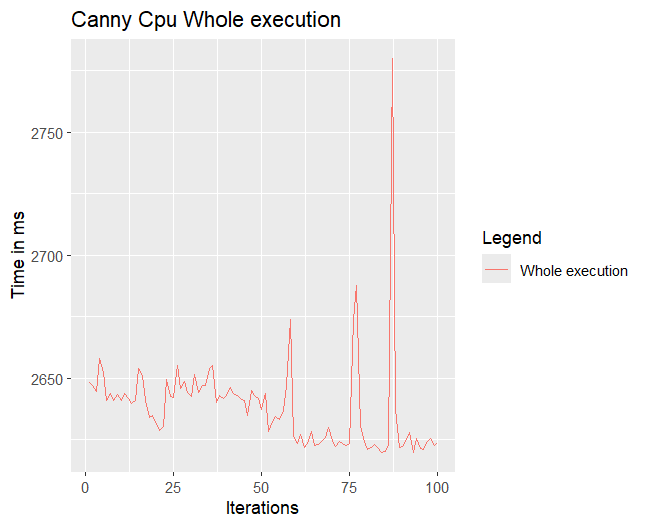
\includegraphics[width=\linewidth]{stest1/canny_cpu_w}
\end{minipage}
\begin{minipage}[t]{.49\textwidth}
\centering
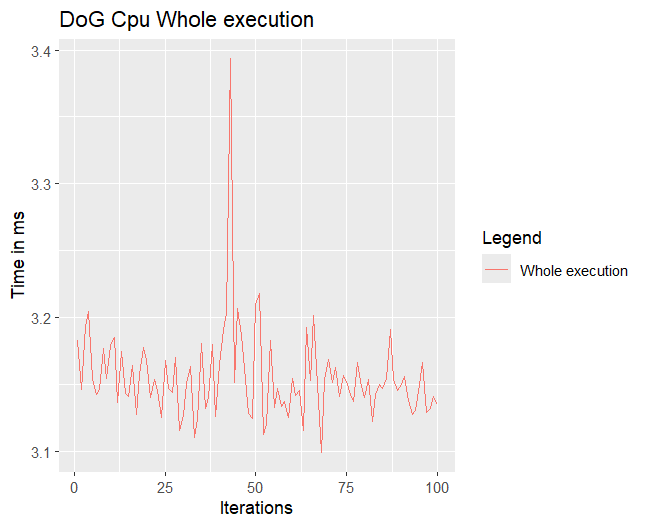
\includegraphics[width=\linewidth]{stest1/dog_cpu_w}
\end{minipage}
\begin{minipage}[t]{.49\textwidth}
\centering
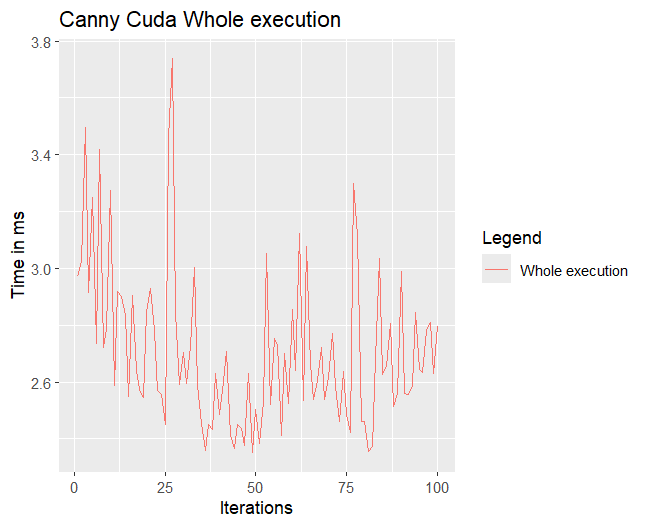
\includegraphics[width=\linewidth]{stest1/canny_cuda_w}
\end{minipage}
\begin{minipage}[t]{.49\textwidth}
\centering
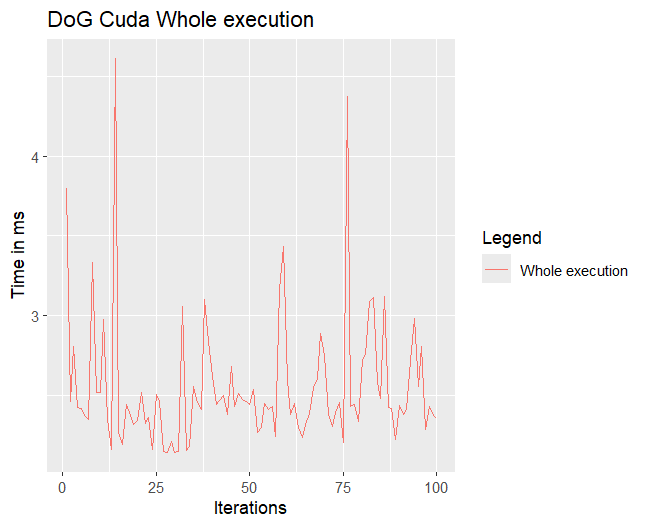
\includegraphics[width=\linewidth]{stest1/dog_cuda_w}
\end{minipage}
\begin{minipage}[t]{.49\textwidth}
\centering
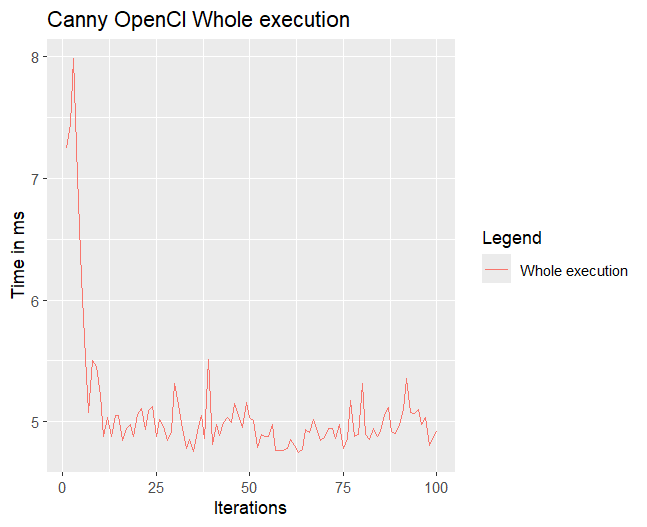
\includegraphics[width=\linewidth]{stest1/canny_open_cl_w}
\end{minipage}
\begin{minipage}[t]{.49\textwidth}
\centering
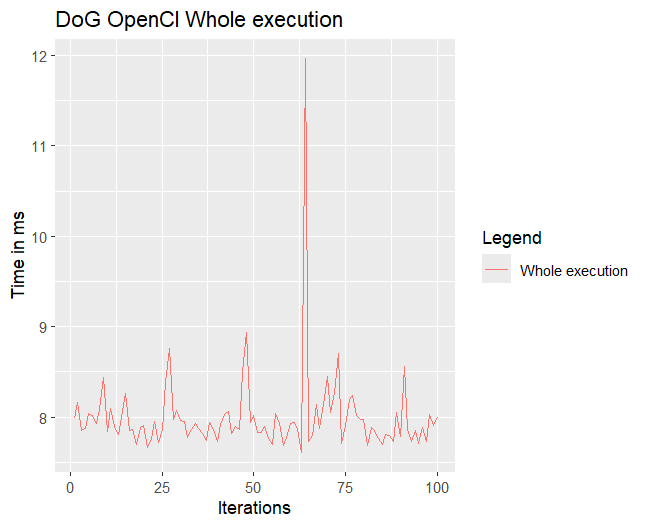
\includegraphics[width=\linewidth]{stest1/dog_open_cl_w}
\end{minipage}
\caption{Graphs for the first synthetic test whole execution time machine1}
\label{fig:test1sw}
\end{figure}

\begin{figure}[H]
\centering
\begin{minipage}[t]{.49\textwidth}
\centering
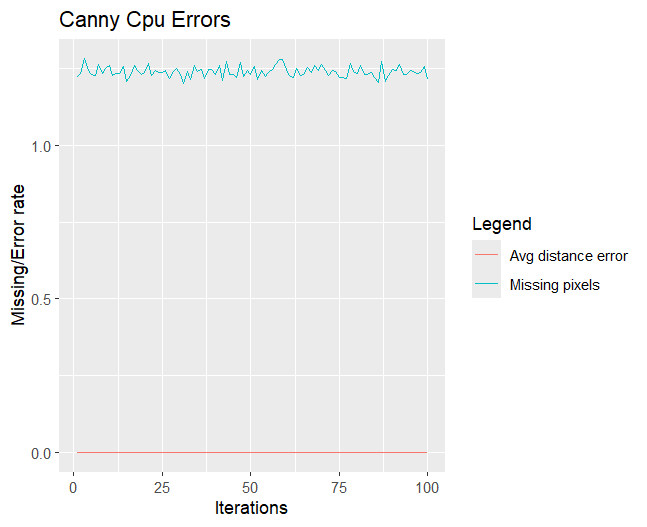
\includegraphics[width=\linewidth]{stest1/canny_cpu_e}
\end{minipage}
\begin{minipage}[t]{.49\textwidth}
\centering
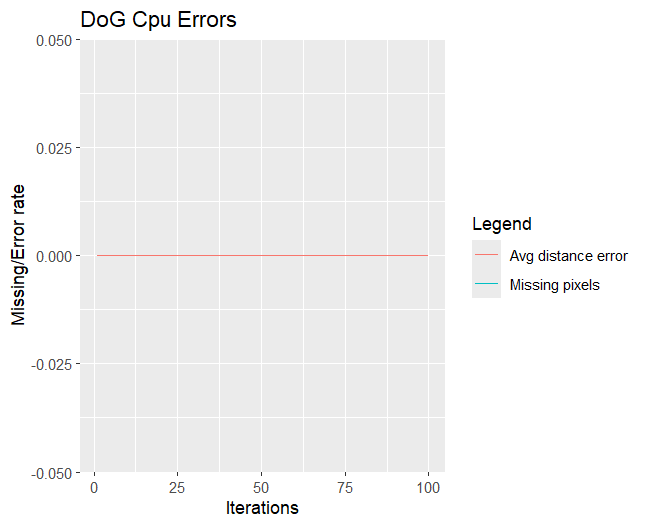
\includegraphics[width=\linewidth]{stest1/dog_cpu_e}
\end{minipage}
\begin{minipage}[t]{.49\textwidth}
\centering
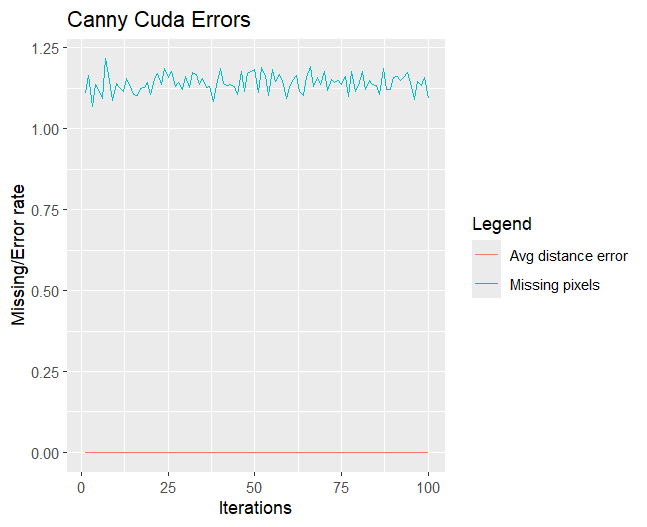
\includegraphics[width=\linewidth]{stest1/canny_cuda_e}
\end{minipage}
\begin{minipage}[t]{.49\textwidth}
\centering
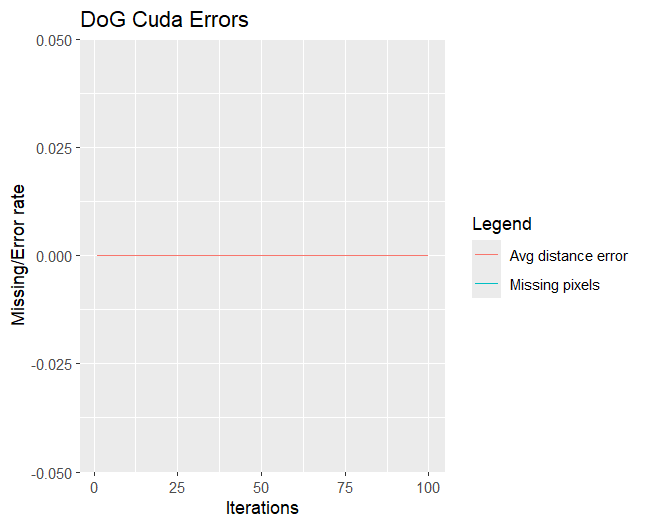
\includegraphics[width=\linewidth]{stest1/dog_cuda_e}
\end{minipage}
\begin{minipage}[t]{.49\textwidth}
\centering
\includegraphics[width=\linewidth]{stest1/canny_open_cl_e}
\end{minipage}
\begin{minipage}[t]{.49\textwidth}
\centering
\includegraphics[width=\linewidth]{stest1/dog_open_cl_e}
\end{minipage}
\caption{Graphs for the first synthetic test results error rate and missing rate machine1}
\label{fig:test1se}
\end{figure}

\begin{figure}[H]
\centering
\begin{minipage}[t]{.49\textwidth}
\centering
\includegraphics[width=\linewidth]{stest1linux/canny_cpu}
\end{minipage}
\begin{minipage}[t]{.49\textwidth}
\centering
\includegraphics[width=\linewidth]{stest1linux/dog_cpu}
\end{minipage}
\begin{minipage}[t]{.49\textwidth}
\centering
\includegraphics[width=\linewidth]{stest1linux/canny_cuda}
\end{minipage}
\begin{minipage}[t]{.49\textwidth}
\centering
\includegraphics[width=\linewidth]{stest1linux/dog_cuda}
\end{minipage}
\begin{minipage}[t]{.49\textwidth}
\centering
\includegraphics[width=\linewidth]{stest1linux/canny_open_cl}
\end{minipage}
\begin{minipage}[t]{.49\textwidth}
\centering
\includegraphics[width=\linewidth]{stest1linux/dog_open_cl}
\end{minipage}
\caption{Graphs for the first synthetic test results on machine2}
\label{fig:test1sl}
\end{figure}

\begin{figure}[H]
\centering
\begin{minipage}[t]{.49\textwidth}
\centering
\includegraphics[width=\linewidth]{stest1linux/canny_cpu_w}
\end{minipage}
\begin{minipage}[t]{.49\textwidth}
\centering
\includegraphics[width=\linewidth]{stest1linux/dog_cpu_w}
\end{minipage}
\begin{minipage}[t]{.49\textwidth}
\centering
\includegraphics[width=\linewidth]{stest1linux/canny_cuda_w}
\end{minipage}
\begin{minipage}[t]{.49\textwidth}
\centering
\includegraphics[width=\linewidth]{stest1linux/dog_cuda_w}
\end{minipage}
\begin{minipage}[t]{.49\textwidth}
\centering
\includegraphics[width=\linewidth]{stest1linux/canny_open_cl_w}
\end{minipage}
\begin{minipage}[t]{.49\textwidth}
\centering
\includegraphics[width=\linewidth]{stest1linux/dog_open_cl_w}
\end{minipage}
\caption{Graphs for the first synthetic test whole execution time on machine2}
\label{fig:test1swl}
\end{figure}

\begin{figure}[H]
\centering
\begin{minipage}[t]{.49\textwidth}
\centering
\includegraphics[width=\linewidth]{stest1linux/canny_cpu_e}
\end{minipage}
\begin{minipage}[t]{.49\textwidth}
\centering
\includegraphics[width=\linewidth]{stest1linux/dog_cpu_e}
\end{minipage}
\begin{minipage}[t]{.49\textwidth}
\centering
\includegraphics[width=\linewidth]{stest1linux/canny_cuda_e}
\end{minipage}
\begin{minipage}[t]{.49\textwidth}
\centering
\includegraphics[width=\linewidth]{stest1linux/dog_cuda_e}
\end{minipage}
\begin{minipage}[t]{.49\textwidth}
\centering
\includegraphics[width=\linewidth]{stest1linux/canny_open_cl_e}
\end{minipage}
\begin{minipage}[t]{.49\textwidth}
\centering
\includegraphics[width=\linewidth]{stest1linux/dog_open_cl_e}
\end{minipage}
\caption{Graphs for the first synthetic test results error rate and missing rate on machine2}
\label{fig:test1sel}
\end{figure}

As seen in \autoref{fig:test1s} and \autoref{fig:test1sl} some of the time especially in the Cuda version there's a huge spike in the time it took to complete the algorithm. I expect this to be because the Cuda timing function puts events into the queue so its not completely exact timing and if the \ac{GPU}'s scheduler decides to work on an other process and not my program the timing will be strange. While on the OpenCl version the documentation doesn't explain how it captures the timing but I have a guess that its in the same process and not in a queue like on Cuda thus the \ac{GPU}'s scheduler cannot influence the timings this is why it's timings are less spiky. 

Still if we compare the timings its clear that the Cuda and the OpenCl version is very close when it comes to how long it took to finish. While the \ac{CPU} version fall of rapidly. Its interesting to note that while the OpenCl version is faster than the Cuda version if we factor in the whole execution in \autoref{fig:test1sw} and \autoref{fig:test1swl} the Cuda version is almost always finishes faster.

Looking at \autoref{fig:test1se} and \autoref{fig:test1sel} its clear that the \ac{DoG} algorithm always finds the pixels perfectly and makes no mistakes every existing pixel has a match. On the other hand looking at the \ac{Canny} version it's clear that it doesn't find all the pixels exactly that's because the \ac{Canny} algorithm finds edges by transitions that means it cannot find a single line on a picture exactly but as the error rate show they are at most two pixels away.

\clearpage

\begin{figure}[H]
\centering
\begin{minipage}[t]{.49\textwidth}
\centering
\includegraphics[width=\linewidth]{stest2/canny_cpu}
\end{minipage}
\begin{minipage}[t]{.49\textwidth}
\centering
\includegraphics[width=\linewidth]{stest2/dog_cpu}
\end{minipage}
\begin{minipage}[t]{.49\textwidth}
\centering
\includegraphics[width=\linewidth]{stest2/canny_cuda}
\end{minipage}
\begin{minipage}[t]{.49\textwidth}
\centering
\includegraphics[width=\linewidth]{stest2/dog_cuda}
\end{minipage}
\begin{minipage}[t]{.49\textwidth}
\centering
\includegraphics[width=\linewidth]{stest2/canny_open_cl}
\end{minipage}
\begin{minipage}[t]{.49\textwidth}
\centering
\includegraphics[width=\linewidth]{stest2/dog_open_cl}
\end{minipage}
\caption{Graphs for the second synthetic test results on machine1}
\label{fig:test2s}
\end{figure}

\begin{figure}[H]
\centering
\begin{minipage}[t]{.49\textwidth}
\centering
\includegraphics[width=\linewidth]{stest2/canny_cpu_w}
\end{minipage}
\begin{minipage}[t]{.49\textwidth}
\centering
\includegraphics[width=\linewidth]{stest2/dog_cpu_w}
\end{minipage}
\begin{minipage}[t]{.49\textwidth}
\centering
\includegraphics[width=\linewidth]{stest2/canny_cuda_w}
\end{minipage}
\begin{minipage}[t]{.49\textwidth}
\centering
\includegraphics[width=\linewidth]{stest2/dog_cuda_w}
\end{minipage}
\begin{minipage}[t]{.49\textwidth}
\centering
\includegraphics[width=\linewidth]{stest2/canny_open_cl_w}
\end{minipage}
\begin{minipage}[t]{.49\textwidth}
\centering
\includegraphics[width=\linewidth]{stest2/dog_open_cl_w}
\end{minipage}
\caption{Graphs for the second synthetic test whole execution time machine1}
\label{fig:test2sw}
\end{figure}

\begin{figure}[H]
\centering
\begin{minipage}[t]{.49\textwidth}
\centering
\includegraphics[width=\linewidth]{stest2/canny_cpu_e}
\end{minipage}
\begin{minipage}[t]{.49\textwidth}
\centering
\includegraphics[width=\linewidth]{stest2/dog_cpu_e}
\end{minipage}
\begin{minipage}[t]{.49\textwidth}
\centering
\includegraphics[width=\linewidth]{stest2/canny_cuda_e}
\end{minipage}
\begin{minipage}[t]{.49\textwidth}
\centering
\includegraphics[width=\linewidth]{stest2/dog_cuda_e}
\end{minipage}
\begin{minipage}[t]{.49\textwidth}
\centering
\includegraphics[width=\linewidth]{stest2/canny_open_cl_e}
\end{minipage}
\begin{minipage}[t]{.49\textwidth}
\centering
\includegraphics[width=\linewidth]{stest2/dog_open_cl_e}
\end{minipage}
\caption{Graphs for the second synthetic test results error rate and missing rate machine1}
\label{fig:test2se}
\end{figure}

\begin{figure}[H]
\centering
\begin{minipage}[t]{.49\textwidth}
\centering
\includegraphics[width=\linewidth]{stest2linux/canny_cpu}
\end{minipage}
\begin{minipage}[t]{.49\textwidth}
\centering
\includegraphics[width=\linewidth]{stest2linux/dog_cpu}
\end{minipage}
\begin{minipage}[t]{.49\textwidth}
\centering
\includegraphics[width=\linewidth]{stest2linux/canny_cuda}
\end{minipage}
\begin{minipage}[t]{.49\textwidth}
\centering
\includegraphics[width=\linewidth]{stest2linux/dog_cuda}
\end{minipage}
\begin{minipage}[t]{.49\textwidth}
\centering
\includegraphics[width=\linewidth]{stest2linux/canny_open_cl}
\end{minipage}
\begin{minipage}[t]{.49\textwidth}
\centering
\includegraphics[width=\linewidth]{stest2/dog_open_cl}
\end{minipage}
\caption{Graphs for the second synthetic test results on machine2}
\label{fig:test2sl}
\end{figure}

\begin{figure}[H]
\centering
\begin{minipage}[t]{.49\textwidth}
\centering
\includegraphics[width=\linewidth]{stest2linux/canny_cpu_w}
\end{minipage}
\begin{minipage}[t]{.49\textwidth}
\centering
\includegraphics[width=\linewidth]{stest2linux/dog_cpu_w}
\end{minipage}
\begin{minipage}[t]{.49\textwidth}
\centering
\includegraphics[width=\linewidth]{stest2linux/canny_cuda_w}
\end{minipage}
\begin{minipage}[t]{.49\textwidth}
\centering
\includegraphics[width=\linewidth]{stest2linux/dog_cuda_w}
\end{minipage}
\begin{minipage}[t]{.49\textwidth}
\centering
\includegraphics[width=\linewidth]{stest2linux/canny_open_cl_w}
\end{minipage}
\begin{minipage}[t]{.49\textwidth}
\centering
\includegraphics[width=\linewidth]{stest2linux/dog_open_cl_w}
\end{minipage}
\caption{Graphs for the second synthetic test whole execution time on machine2}
\label{fig:test2swl}
\end{figure}

\begin{figure}[H]
\centering
\begin{minipage}[t]{.49\textwidth}
\centering
\includegraphics[width=\linewidth]{stest2linux/canny_cpu_e}
\end{minipage}
\begin{minipage}[t]{.49\textwidth}
\centering
\includegraphics[width=\linewidth]{stest2linux/dog_cpu_e}
\end{minipage}
\begin{minipage}[t]{.49\textwidth}
\centering
\includegraphics[width=\linewidth]{stest2linux/canny_cuda_e}
\end{minipage}
\begin{minipage}[t]{.49\textwidth}
\centering
\includegraphics[width=\linewidth]{stest2linux/dog_cuda_e}
\end{minipage}
\begin{minipage}[t]{.49\textwidth}
\centering
\includegraphics[width=\linewidth]{stest2linux/canny_open_cl_e}
\end{minipage}
\begin{minipage}[t]{.49\textwidth}
\centering
\includegraphics[width=\linewidth]{stest2linux/dog_open_cl_e}
\end{minipage}
\caption{Graphs for the second synthetic test results error rate and missing rate on machine2}
\label{fig:test2sel}
\end{figure}

Comparing the results of the first test with the results from the second test in \autoref{fig:test2s} and \autoref{fig:test2sl} its clear that while the size of the image matters in terms of how long it takes it isn't the deciding factor. The most time goes to the convolution done with the gauss kernel named blur and convolution respectively in the two algorithms.

But looking at the errors in \autoref{fig:test2se} and \autoref{fig:test2sel} no matter the size of the picture or the kernel the errors are just like in the first test. In the next two test lets see if increasing the lines count will produce more errors or not.

\begin{figure}[H]
\centering
\begin{minipage}[t]{.49\textwidth}
\centering
\includegraphics[width=\linewidth]{stest3/canny_cpu}
\end{minipage}
\begin{minipage}[t]{.49\textwidth}
\centering
\includegraphics[width=\linewidth]{stest3/dog_cpu}
\end{minipage}
\begin{minipage}[t]{.49\textwidth}
\centering
\includegraphics[width=\linewidth]{stest3/canny_cuda}
\end{minipage}
\begin{minipage}[t]{.49\textwidth}
\centering
\includegraphics[width=\linewidth]{stest3/dog_cuda}
\end{minipage}
\begin{minipage}[t]{.49\textwidth}
\centering
\includegraphics[width=\linewidth]{stest3/canny_open_cl}
\end{minipage}
\begin{minipage}[t]{.49\textwidth}
\centering
\includegraphics[width=\linewidth]{stest3/dog_open_cl}
\end{minipage}
\caption{Graphs for the third synthetic test results on machine1}
\label{fig:test3s}
\end{figure}

\begin{figure}[H]
\centering
\begin{minipage}[t]{.49\textwidth}
\centering
\includegraphics[width=\linewidth]{stest3/canny_cpu_w}
\end{minipage}
\begin{minipage}[t]{.49\textwidth}
\centering
\includegraphics[width=\linewidth]{stest3/dog_cpu_w}
\end{minipage}
\begin{minipage}[t]{.49\textwidth}
\centering
\includegraphics[width=\linewidth]{stest3/canny_cuda_w}
\end{minipage}
\begin{minipage}[t]{.49\textwidth}
\centering
\includegraphics[width=\linewidth]{stest3/dog_cuda_w}
\end{minipage}
\begin{minipage}[t]{.49\textwidth}
\centering
\includegraphics[width=\linewidth]{stest3/canny_open_cl_w}
\end{minipage}
\begin{minipage}[t]{.49\textwidth}
\centering
\includegraphics[width=\linewidth]{stest3/dog_open_cl_w}
\end{minipage}
\caption{Graphs for the third synthetic test whole execution time machine1}
\label{fig:test3sw}
\end{figure}

\begin{figure}[H]
\centering
\begin{minipage}[t]{.49\textwidth}
\centering
\includegraphics[width=\linewidth]{stest3/canny_cpu_e}
\end{minipage}
\begin{minipage}[t]{.49\textwidth}
\centering
\includegraphics[width=\linewidth]{stest3/dog_cpu_e}
\end{minipage}
\begin{minipage}[t]{.49\textwidth}
\centering
\includegraphics[width=\linewidth]{stest3/canny_cuda_e}
\end{minipage}
\begin{minipage}[t]{.49\textwidth}
\centering
\includegraphics[width=\linewidth]{stest3/dog_cuda_e}
\end{minipage}
\begin{minipage}[t]{.49\textwidth}
\centering
\includegraphics[width=\linewidth]{stest3/canny_open_cl_e}
\end{minipage}
\begin{minipage}[t]{.49\textwidth}
\centering
\includegraphics[width=\linewidth]{stest3/dog_open_cl_e}
\end{minipage}
\caption{Graphs for the third synthetic test results error rate and missing rate machine1}
\label{fig:test3se}
\end{figure}

\begin{figure}[H]
\centering
\begin{minipage}[t]{.49\textwidth}
\centering
\includegraphics[width=\linewidth]{stest4/canny_cpu}
\end{minipage}
\begin{minipage}[t]{.49\textwidth}
\centering
\includegraphics[width=\linewidth]{stest4/dog_cpu}
\end{minipage}
\begin{minipage}[t]{.49\textwidth}
\centering
\includegraphics[width=\linewidth]{stest4/canny_cuda}
\end{minipage}
\begin{minipage}[t]{.49\textwidth}
\centering
\includegraphics[width=\linewidth]{stest4/dog_cuda}
\end{minipage}
\begin{minipage}[t]{.49\textwidth}
\centering
\includegraphics[width=\linewidth]{stest4/canny_open_cl}
\end{minipage}
\begin{minipage}[t]{.49\textwidth}
\centering
\includegraphics[width=\linewidth]{stest4/dog_open_cl}
\end{minipage}
\caption{Graphs for the forth synthetic test results on machine1}
\label{fig:test4s}
\end{figure}

\begin{figure}[H]
\centering
\begin{minipage}[t]{.49\textwidth}
\centering
\includegraphics[width=\linewidth]{stest4/canny_cpu_w}
\end{minipage}
\begin{minipage}[t]{.49\textwidth}
\centering
\includegraphics[width=\linewidth]{stest4/dog_cpu_w}
\end{minipage}
\begin{minipage}[t]{.49\textwidth}
\centering
\includegraphics[width=\linewidth]{stest4/canny_cuda_w}
\end{minipage}
\begin{minipage}[t]{.49\textwidth}
\centering
\includegraphics[width=\linewidth]{stest4/dog_cuda_w}
\end{minipage}
\begin{minipage}[t]{.49\textwidth}
\centering
\includegraphics[width=\linewidth]{stest4/canny_open_cl_w}
\end{minipage}
\begin{minipage}[t]{.49\textwidth}
\centering
\includegraphics[width=\linewidth]{stest4/dog_open_cl_w}
\end{minipage}
\caption{Graphs for the forth synthetic test whole execution time machine1}
\label{fig:tes4sw}
\end{figure}

\begin{figure}[H]
\centering
\begin{minipage}[t]{.49\textwidth}
\centering
\includegraphics[width=\linewidth]{stest4/canny_cpu_e}
\end{minipage}
\begin{minipage}[t]{.49\textwidth}
\centering
\includegraphics[width=\linewidth]{stest4/dog_cpu_e}
\end{minipage}
\begin{minipage}[t]{.49\textwidth}
\centering
\includegraphics[width=\linewidth]{stest4/canny_cuda_e}
\end{minipage}
\begin{minipage}[t]{.49\textwidth}
\centering
\includegraphics[width=\linewidth]{stest4/dog_cuda_e}
\end{minipage}
\begin{minipage}[t]{.49\textwidth}
\centering
\includegraphics[width=\linewidth]{stest4/canny_open_cl_e}
\end{minipage}
\begin{minipage}[t]{.49\textwidth}
\centering
\includegraphics[width=\linewidth]{stest4/dog_open_cl_e}
\end{minipage}
\caption{Graphs for the forth synthetic test results error rate and missing rate machine1}
\label{fig:test4se}
\end{figure}

Looking at the results of the third and forth tests in \autoref{fig:test3s} and \autoref{fig:test4s} its clear that the time it takes for the algorithm to finish is not influenced by what is present on the pictures.
At the same time in \autoref{fig:test3se} and \autoref{fig:test4se} the error rates are the same a little higher maybe but that's well within the range of error thus we can conclude that having more things on a picture does not results in more errors.